%%=============================================================================
%% Verwerking resultaten
%%=============================================================================

\chapter{Verwerking resultaten}
\label{ch:Verwerking resultaten}

%inleiding tot hoofdstuk
In dit hoofdstuk zullen de verschillende resultaten van de requirementanalyse van de oplossingen verwerkt worden om zo tot een statistisch correct antwoord te komen op de hoofdonderzoeksvraag uit Sectie~\ref{subsec:Hoofdonderzoeksvraag}.

\section{\IfLanguageName{dutch}{Resultaten requirements}{Resultaten requirements}}
\label{sec:Resultaten requirements}

%Tabel met gemiddelde/Mediaan/Modus/Standaardafwijking/variatiecoefficientie
%En dan verwerking resultaten gelik bij Thomas zijn BAP

%In onderstaande tabellen wordt de onderverdeling van de punten van de verschillende oplossingen duidelijk gemaakt. Bij “Must have” zijn er 3 items waar per item 5 punten te verdienen zijn. “Should have” kent 2 items, die samen voor 5 punten meetellen (2 x 2.5). De “Could have” items worden niet meegerekend omdat deze van geen belang zijn geweest in de keuze naar een oplossing. Het totaal van de punten staat op 20. De twee oplossingen met de hoogste score zullen gebruikt worden voor een nog meer verdiepende studie die meer in detail gaat bij deze twee oplossingen. De oplossing met de hoogste score zal ook gebruikt worden bij het opzetten van de proof-of-concept.

Hieronder vindt u per PostgreSQL High Availability cluster oplossing een overzicht van het gemiddelde, de mediaan, de modus, de standaardafwijking en de variatiecoëfficiënt van alle scores gegeven op de requirements.

\begin{table}[!h]
    \centering
    \resizebox{\textwidth}{!}{%
        \begin{tabular}{|l|c|c|c|c|}
            \hline
            \multicolumn{1}{|r|}{} & Patroni & PostgreSQL Automatic Failover (PAF) & Pgpool-II & Replication Manager (repmgr) \\ \hline
            Gemiddelde          & 4.4 & 4,2 & 3,8 & /4 \\ \hline
            Mediaan             & 4 & 4 & 4 & 4 \\ \hline
            Modus               & 4 & 4 & 3 \& 4 & 4 \\ \hline
            Standaardafwijking  & 0,55 & 0,45 & 0,84 & 0,71 \\ \hline
            Variatiecoëfficiënt & 0,12 & 0,11 & 0,22 & 0,18 \\ \hline
        \end{tabular}%
    }
    \caption{Statistieken requirements}
    \label{table:Statistieken requirements}
\end{table}

Om deze resultaten met elkaar te vergelijken, wordt er gebruik gemaakt van niet-gepaarde t-testen.





Bovenstaande resultaten werden behaald met onderstaande code in R. Hierin werd telkens het gemiddelde, de mediaan, de modus, de standaardafwijking en de variatiecoëfficiënt berekend.

\begin{figure}[!h]
    \centering
    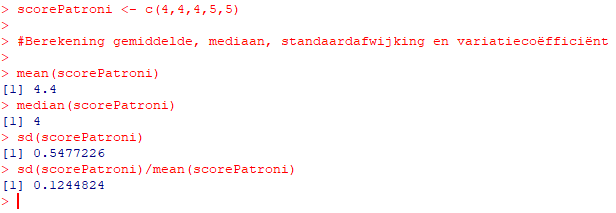
\includegraphics[width=\linewidth]{PatroniR.png}
    \caption{R berekening voor Patroni}
    \label{fig:R berekening voor Patroni}
\end{figure}

\begin{figure}[!h]
    \centering
    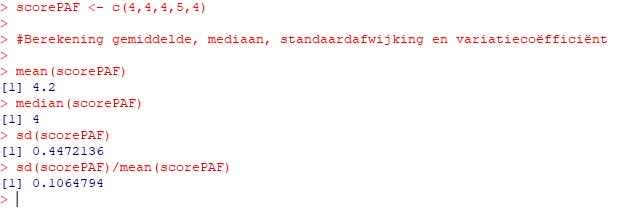
\includegraphics[width=\linewidth]{PAFR.png}
    \caption{R berekening voor PostgreSQL Automatic Failover (PAF)}
    \label{fig:R berekening voor PostgreSQL Automatic Failover (PAF)}
\end{figure}

\begin{figure}[!h]
    \centering
    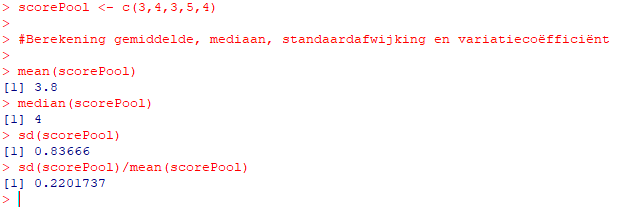
\includegraphics[width=\linewidth]{PoolR.png}
    \caption{R berekening voor Pgpool-II}
    \label{fig:R berekening voor Pgpool-II}
\end{figure}

\begin{figure}[!h]
    \centering
    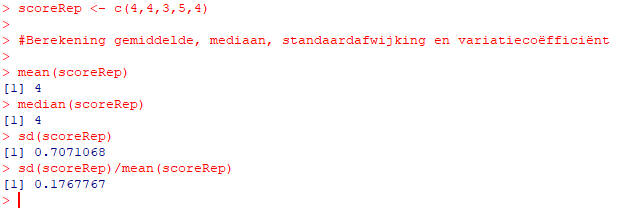
\includegraphics[width=\linewidth]{RepR.png}
    \caption{R berekening voor Replication Manager (repmgr)}
    \label{fig:R berekening voor Replication Manager (repmgr)}
\end{figure}

\begin{figure}[!h]
    \centering
    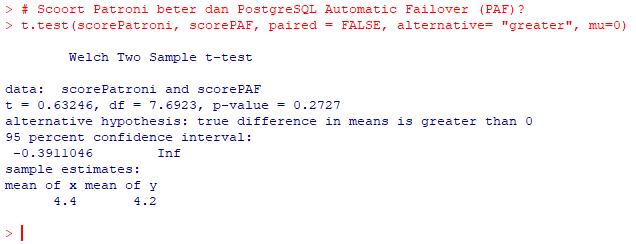
\includegraphics[width=\linewidth]{PatroniVSPAF.png}
    \caption{R berekening Patroni en PostgreSQL Automatic Failover (PAF)}
    \label{fig:R berekening Patroni en PostgreSQL Automatic Failover (PAF)}
\end{figure}

\begin{figure}[!h]
    \centering
    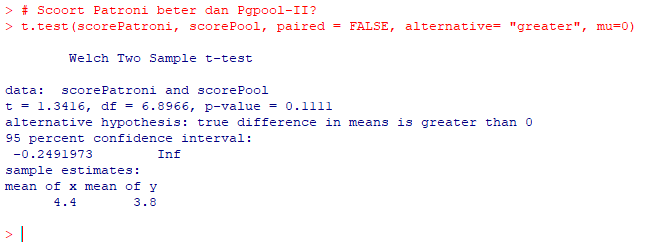
\includegraphics[width=\linewidth]{PatroniVSPool.png}
    \caption{R berekening Patroni en Pgpool-II}
    \label{fig:R berekening Patroni en Pgpool-II}
\end{figure}

\begin{figure}[!h]
    \centering
    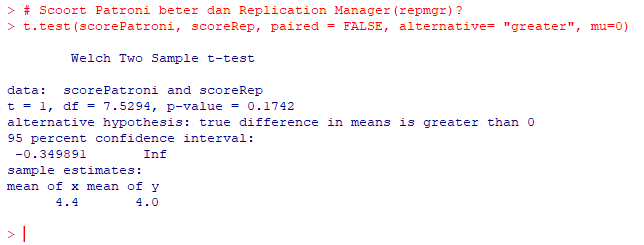
\includegraphics[width=\linewidth]{PatroniVSRep.png}
    \caption{R berekening Patroni en Replication Manager (repmgr)}
    \label{fig:R berekening Patroni en Replication Manager (repmgr)}
\end{figure}

\begin{figure}[!h]
    \centering
    \includegraphics[width=\linewidth]{PAFVSPool.png}
    \caption{R berekening PostgreSQL Automatic Failover (PAF) en Pgpool-II}
    \label{fig:R berekening PostgreSQL Automatic Failover (PAF) en Pgpool-II}
\end{figure}

\begin{figure}[!h]
    \centering
    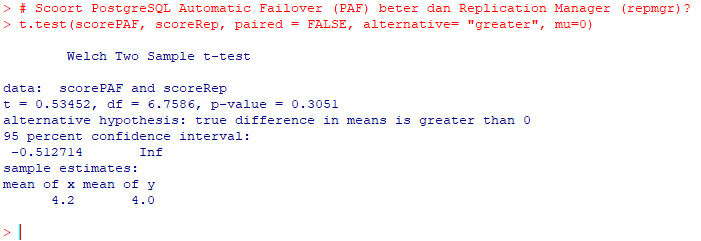
\includegraphics[width=\linewidth]{PAFVSRep.png}
    \caption{R berekening PostgreSQL Automatic Failover (PAF) en Replication Manager (repmgr)}
    \label{fig:R berekening PostgreSQL Automatic Failover (PAF) en Replication Manager (repmgr)}
\end{figure}

\begin{figure}[!h]
    \centering
    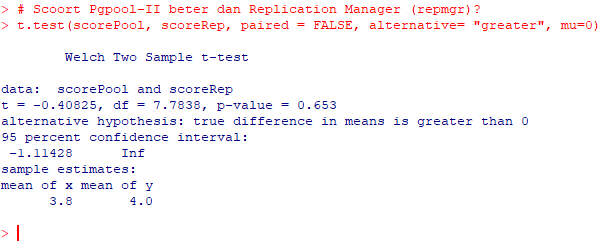
\includegraphics[width=\linewidth]{RepVSPool.png}
    \caption{R berekening Replication Manager (repmgr) en Pgpool-II}
    \label{fig:R berekening Replication Manager (repmgr) en Pgpool-II}
\end{figure}



%\begin{table}[!h]
%    \centering
%    \begin{tabular}{ |p{6cm}||p{6cm}|  }
%        \hline
%        \multicolumn{2}{|c|}{Requirementanalyse Alle Oplossingen} \\
%        \hline
%        Patroni & 17/20 \\
%        \hline
%        Pgpool-II & 14/20 \\
%        \hline
%        PostgreSQL Automatic Failover (PAF) & 16/20 \\
%        \hline
%        Replication Manager (repmgr) & 15/20 \\
%        \hline
%    \end{tabular}
%    \caption{Requirementanalyse alle oplossingen}
%    \label{table:Requirementanalyse alle oplossingen}
%    In de laatste tabel is er een duidelijke onderverdeling in score van de oplossingen. In dit onderzoek zal verder verdiept worden in Patroni en PostgreSQL Automatic Failover en bijhorende tools. Voor proof of concept zal gebruik worden gemaakt van Patroni.
%\end{table}



